\section{Experiments} % Ukazka toho, jak presny je pointcloud ze skeneru

We explore the rendering performance of various renderers used in the thesis,
both in terms of the rendering quality compared to the respective real image
and the actual time it takes to render an image of a given size. Underlying
dependency on point cloud density is also touched. Finally, the influence of the
renderers used for pose verification in the InLoc localization pipeline is examined.


\subsection{Comparison of renderers}

For \textbf{statistical comparison} of an RGB rendering produced by
given renderer to the
respective real-world image captured by a camera, we utilize two
metrics---pixel-wise $L_1$ loss and Peak Signal to Noise Ratio (PSNR). The final metric
value across a dataset is computed as the mean value of the loss per photo.

\def\m{~\mathrm{m}}
\def\M{\mathrm{m}}
\def\dg{^{\circ}}
\def\D{\phantom{0}}
\def\B{\textbf}
\begin{table}[hb]
\caption[Comparison of $L_1$ and PSNR metrics over Hagia Sophia collection]{
Comparison of $L_1$ (the smaller, the better) and PSNR (the bigger the
better) metrics over the IMC Hagia Sophia collection. For the neural models,
the point cloud of a given density is used for training and inference. Column
Renderer uses notation \emph{P} (Pyrender), \emph{S} (Splatter),
\emph{M} (Marcher), and three \emph{N} variants standing for NRIW trained
on the respective renderer.}
\centering
    \begin{tabular}{l c c l S[table-format=3.2] S[table-format=3.2]}
    \toprule
    Dataset & Density [\%] & Points [M] & Renderer & {$L_1$} & {PSNR}\\
    \midrule
    Hagia Sophia & 25  & 1.25 & P   &    39.93  &    13.94  \\
                 &     &      & S   &    43.01  &    13.00  \\
                 &     &      & M   &    35.83  &    14.69  \\
                 &     &      & N-P &    22.66  &    18.62  \\
                 &     &      & N-S & \B{21.80} & \B{18.73} \\
                 &     &      & N-M &    21.99  &    18.67  \\[0.3cm]

                 & 50  & 2.49 & P   &    36.19  &    14.66  \\
                 &     &      & S   &    36.56  &    14.51  \\
                 &     &      & M   &    34.25  &    15.12  \\
                 &     &      & N-P &    21.85  &    18.88  \\
                 &     &      & N-S &    21.20  &    19.01  \\
                 &     &      & N-M & \B{20.78} & \B{19.32} \\[0.3cm]

                 & 100 & 4.98 & P   &    36.04  &    14.70  \\
                 &     &      & S   &    35.11  &    14.91  \\
                 &     &      & M   &    37.19  &    14.37  \\
                 &     &      & N-P & \B{22.37} &    18.78  \\
                 &     &      & N-S &    22.85  & \B{19.29} \\
                 &     &      & N-M &    22.66  &    18.89  \\
    \bottomrule
    \end{tabular}
\label{tab:hagia_rendering_metrics}
\end{table}

Since many models needed to be trained in a considerably costly
process, only Image Matching Challenge data is used. The results can be seen in
tables~\cref{tab:hagia_rendering_metrics}, \cref{tab:grand_rendering_metrics}, 
and \cref{tab:pantheon_rendering_metrics}. We compare not only three non-neural
renderers plus three neural models trained on those renderers' data but
also point cloud density. The density generally affects rendering times for
classical and non-neural renderers and transversely affects complete render
times for a neural model inference.

\begin{table}[h]
\caption[Comparison of $L_1$ and PSNR metrics over Grand Place collection]{
Comparison of $L_1$ (the smaller, the better) and PSNR (the bigger, the
better) metrics over IMC Grand Place collection. For the neural models,
the point cloud of a given density is used for both training and inference.
Column Renderer uses notation \emph{P} (Pyrender), \emph{S} (Splatter),
\emph{M} (Marcher), and three \emph{N} variants standing for NRIW trained
on the respective renderer.}
\centering
    \begin{tabular}{l c c l S[table-format=3.2] S[table-format=3.2]}
    \toprule
    Dataset & Density [\%] & Points [M] & Renderer & {$L_1$} & {PSNR}\\
    \midrule
    Grand Place  & 25  & 1.09 & P   &    60.81  &    10.59  \\
                 &     &      & S   &    38.61  &    14.25  \\
                 &     &      & M   &    39.74  &    14.04  \\
                 &     &      & N-P &    25.33  &    18.23  \\
                 &     &      & N-S &    23.75  & \B{20.01} \\
                 &     &      & N-M & \B{23.82} &    19.94  \\[0.3cm]

                 & 50  & 2.19 & P   &    57.32  &    11.20  \\
                 &     &      & S   &    39.85  &    14.05  \\
                 &     &      & M   &    40.39  &    13.88  \\
                 &     &      & N-P &    26.44  &    17.92  \\
                 &     &      & N-S &    23.21  &    20.12  \\
                 &     &      & N-M & \B{23.05} & \B{20.20} \\[0.3cm]

                 & 100 & 4.37 & P   &    57.33  &    11.23  \\
                 &     &      & S   &    37.85  &    14.52  \\
                 &     &      & M   &    39.90  &    13.74  \\
                 &     &      & N-P &    25.63  &    18.25  \\
                 &     &      & N-S & \B{22.98} &    19.86  \\
                 &     &      & N-M &    23.11  & \B{20.03} \\
    \bottomrule
    \end{tabular}
\label{tab:grand_rendering_metrics}
\end{table}

The metric values for an image pair in the tables are, analogously to
how similarity in the InLoc verification step is computed, determined over
positions of pixels of the rendered image that are not
of the background color.

We can see performance gains from using neural models across the tables.
Further, ray marching and point splatting methods are better than basic
Pyrender, as discussed below. The relative difference also translates to
neural models. It suggests that for methods presented in the thesis, the
difference in the quality of training data used for training notably
positively impacts the NRIW model. It also suggests that it can positively
influence the pose verification step explored further in this chapter.
Splatter and Marcher are very similar in performance, and it cannot be
determined which is better, notably because they work similarly in theory.

There are no such considerable differences between point cloud densities
for the other data dimensions. The absence of substantial metric difference
means that for a given scene/environment it may make sense to explore and use
less than the full number of points if the time needed for producing one virtual
view is essential. For subsequent experiments, in order to reduce the size of
the space explored, we use only full-size point clouds at our disposal.

The biggest difference in $L_1$ metric between Pyrender and other non-neural
renderers visible in data for Grand Place and Pantheon can be again explained
by the screen space point size by which the renderer is parametrized. The size
is almost view-dependent as for different views, there may be different screen
space \verb|GL_POINTS| dimensions needed for getting flat-like surfaces, whereas
for Splatter and Marcher, fixed per-point diameter can be determined, making this
parametrization whole scene-dependent. It is also not that easy to determine
the size in the case of Pyrender programmatically and in the aforementioned
cases, the size was less suitable in total when combining views over the data
as a whole, resulting in occlusion problem with visible points from normally
non-visible parts of the scene that transversely taints metric computation;
this effect is described in~\nameref{intro}. For Splatter and Marcher,
per-point diameters based on nearest neighbors within a given (simplified) point
cloud are used with the 90-th percentile used for maximal point diameter rendered
to filter out outliers that cause huge splats and spheres, respectively. These
outlier points are more prevalent for point clouds generated by SfM and MVS,
compared to scanner-generated ones.\\

\begin{table}
\caption[Comparison of $L_1$ and PSNR metrics over Pantheon Exterior collection]{
Comparison of $L_1$ (the smaller, the better) and PSNR (the bigger, the
better) metrics over IMC Pantheon Exterior collection. For the neural models,
the point cloud of a given density is used for both training and inference. Column
Renderer uses notation \emph{P} (Pyrender), \emph{S} (Splatter),
\emph{M} (Marcher), and three \emph{N} variants standing for NRIW trained
on the respective renderer.}
\centering
    \begin{tabular}{l c c l S[table-format=3.2] S[table-format=3.2]}
    \toprule
    Dataset & Density [\%] & Points [M] & Renderer & {$L_1$} & {PSNR}\\
    \midrule
    Pantheon     & 25  & 1.18 & P   &    50.68  &    11.31  \\
                 &     &      & S   &    38.20  &    14.24  \\
                 &     &      & M   &    39.32  &    13.94  \\
                 &     &      & N-P &    22.87  &    18.91  \\
                 &     &      & N-S & \B{20.35} &    20.65  \\
                 &     &      & N-M &    21.28  & \B{21.00} \\[0.3cm]

                 & 50  & 2.35 & P   &    49.22  &    11.50  \\
                 &     &      & S   &    42.39  &    13.19  \\
                 &     &      & M   &    40.10  &    13.76  \\
                 &     &      & N-P &    23.10  &    18.75  \\
                 &     &      & N-S &    21.04  &    19.94  \\
                 &     &      & N-M & \B{20.99} & \B{20.18} \\[0.3cm]

                 & 100 & 4.70 & P   &    49.16  &    11.53  \\
                 &     &      & S   &    39.06  &    14.07  \\
                 &     &      & M   &    40.67  &    13.64  \\
                 &     &      & N-P &    18.86  &    22.84  \\
                 &     &      & N-S & \B{17.70} & \B{22.92} \\
                 &     &      & N-M &    18.24  &    21.72 \\
    \bottomrule
    \end{tabular}
\label{tab:pantheon_rendering_metrics}
\end{table}

For \textbf{visual comparison}, several dimensions are explored.
In~\cref{fig:pcd_all}, point cloud density visual qualities are
visualized using Pyrender across IMC collections and point cloud
densities explored, with one image example per given image collection.
The point cloud simplification method used for obtaining smaller density
point clouds is the so-called voxel downsampling that should preserve point
cloud structure. The method relies on decimating neighboring points into
one point in the resulting smaller point cloud based on fixed-size volumes called
voxels. The impact on visual representation is noticeable, especially
on the Grand Place render of the lowest density point cloud, as the background
intentionally displayed in contrasting colors shines through the
building uniformly across its facade.

For more complex point clouds with hidden structures behind a camera
facing simple surfaces such as a facade or a boundary of one vast
internal space, such background visibility could easily be substituted by
points of those otherwise non-visible scene portions. The
problem should be resolved by using Splatter and Marcher renderers---it
is, as can be seen on the per-collection example image comparison
matrices~\cref{fig:hagia_renderers}, \cref{fig:grand_renderers}, and
\cref{fig:pantheon_renderers}. Again, for the Pyrender image produced by
the sparsest point cloud, \uv{background} is more visible, especially
in the case of the Grand Place example and in the case of the Pantheon
example, a hidden structure example in the form of a column in front of
the temple. As far as the Hagia Sophia image is concerned, the view depicts
the surface sufficiently far away from the camera, so the background is
not visible in this case. For the two non-neural renderers, the background
visibility problem is, as expected, not present in any visibly excessive
amount. The smaller sparsity influences those as well, though---using
fewer points leads to more blurry renders, as the diameters of the
remaining points are bigger. On the other hand, the rendering is faster
and, as visible, still more continuous. 

The neural rendering approach is represented by just one unspecified
model in~\cref{fig:hagia_renderers}, \cref{fig:grand_renderers}, and
\cref{fig:pantheon_renderers} as visually the results of differently
trained models' outputs are relatively similar; instead, the density
dimension is displayed. The relative differences are illustrated on InLoc
dataset in~\cref{fig:inloc_renderers}. The notable feature of the
neural rendering method is the \emph{ability to fill} (to some extent)
portions of resulting render image without any respective point
information, namely sky or gaps between screen space points, masking
Pyrender's flaws. Splats and spheres are far better, but not perfect,
rendering primitive from this perspective. However, there is always
some space between neighboring elements stemming from the inability
to cover a surface using circular objects with no overlaps or gaps.
A neural renderer can mask those as well. This has an influence on
the pose verification step explored in the following subsections.

\begin{figure}
    \centering
    \includegraphics[width=0.95\textwidth]{graphics/pcd-all}
    \caption[Visual comparison of point cloud density influence on rendering]{
    Visual comparison of point cloud density influence on rendering.
    The renders are produced by Pyrender (\protect\UseVerb{term}) with contrastive
    background color to present the differences better. Point cloud
    simplification is done by Open3D's voxel downsampling to preserve the original
    structure with fewer points. The downsampling method proceeds in two steps;
    firstly, points are bucketed into 3D volumes called \emph{voxels},
    each resulting in exactly one point of the simplified output by averaging
    all points inside the source voxel in the second step. Since Pyrender
    has a fixed point size in screen space, its disadvantage can be seen---closest
    portions of the scene look sparser than the farther portions.}
    \label{fig:pcd_all}
\end{figure}

\begin{figure}
    \centering
    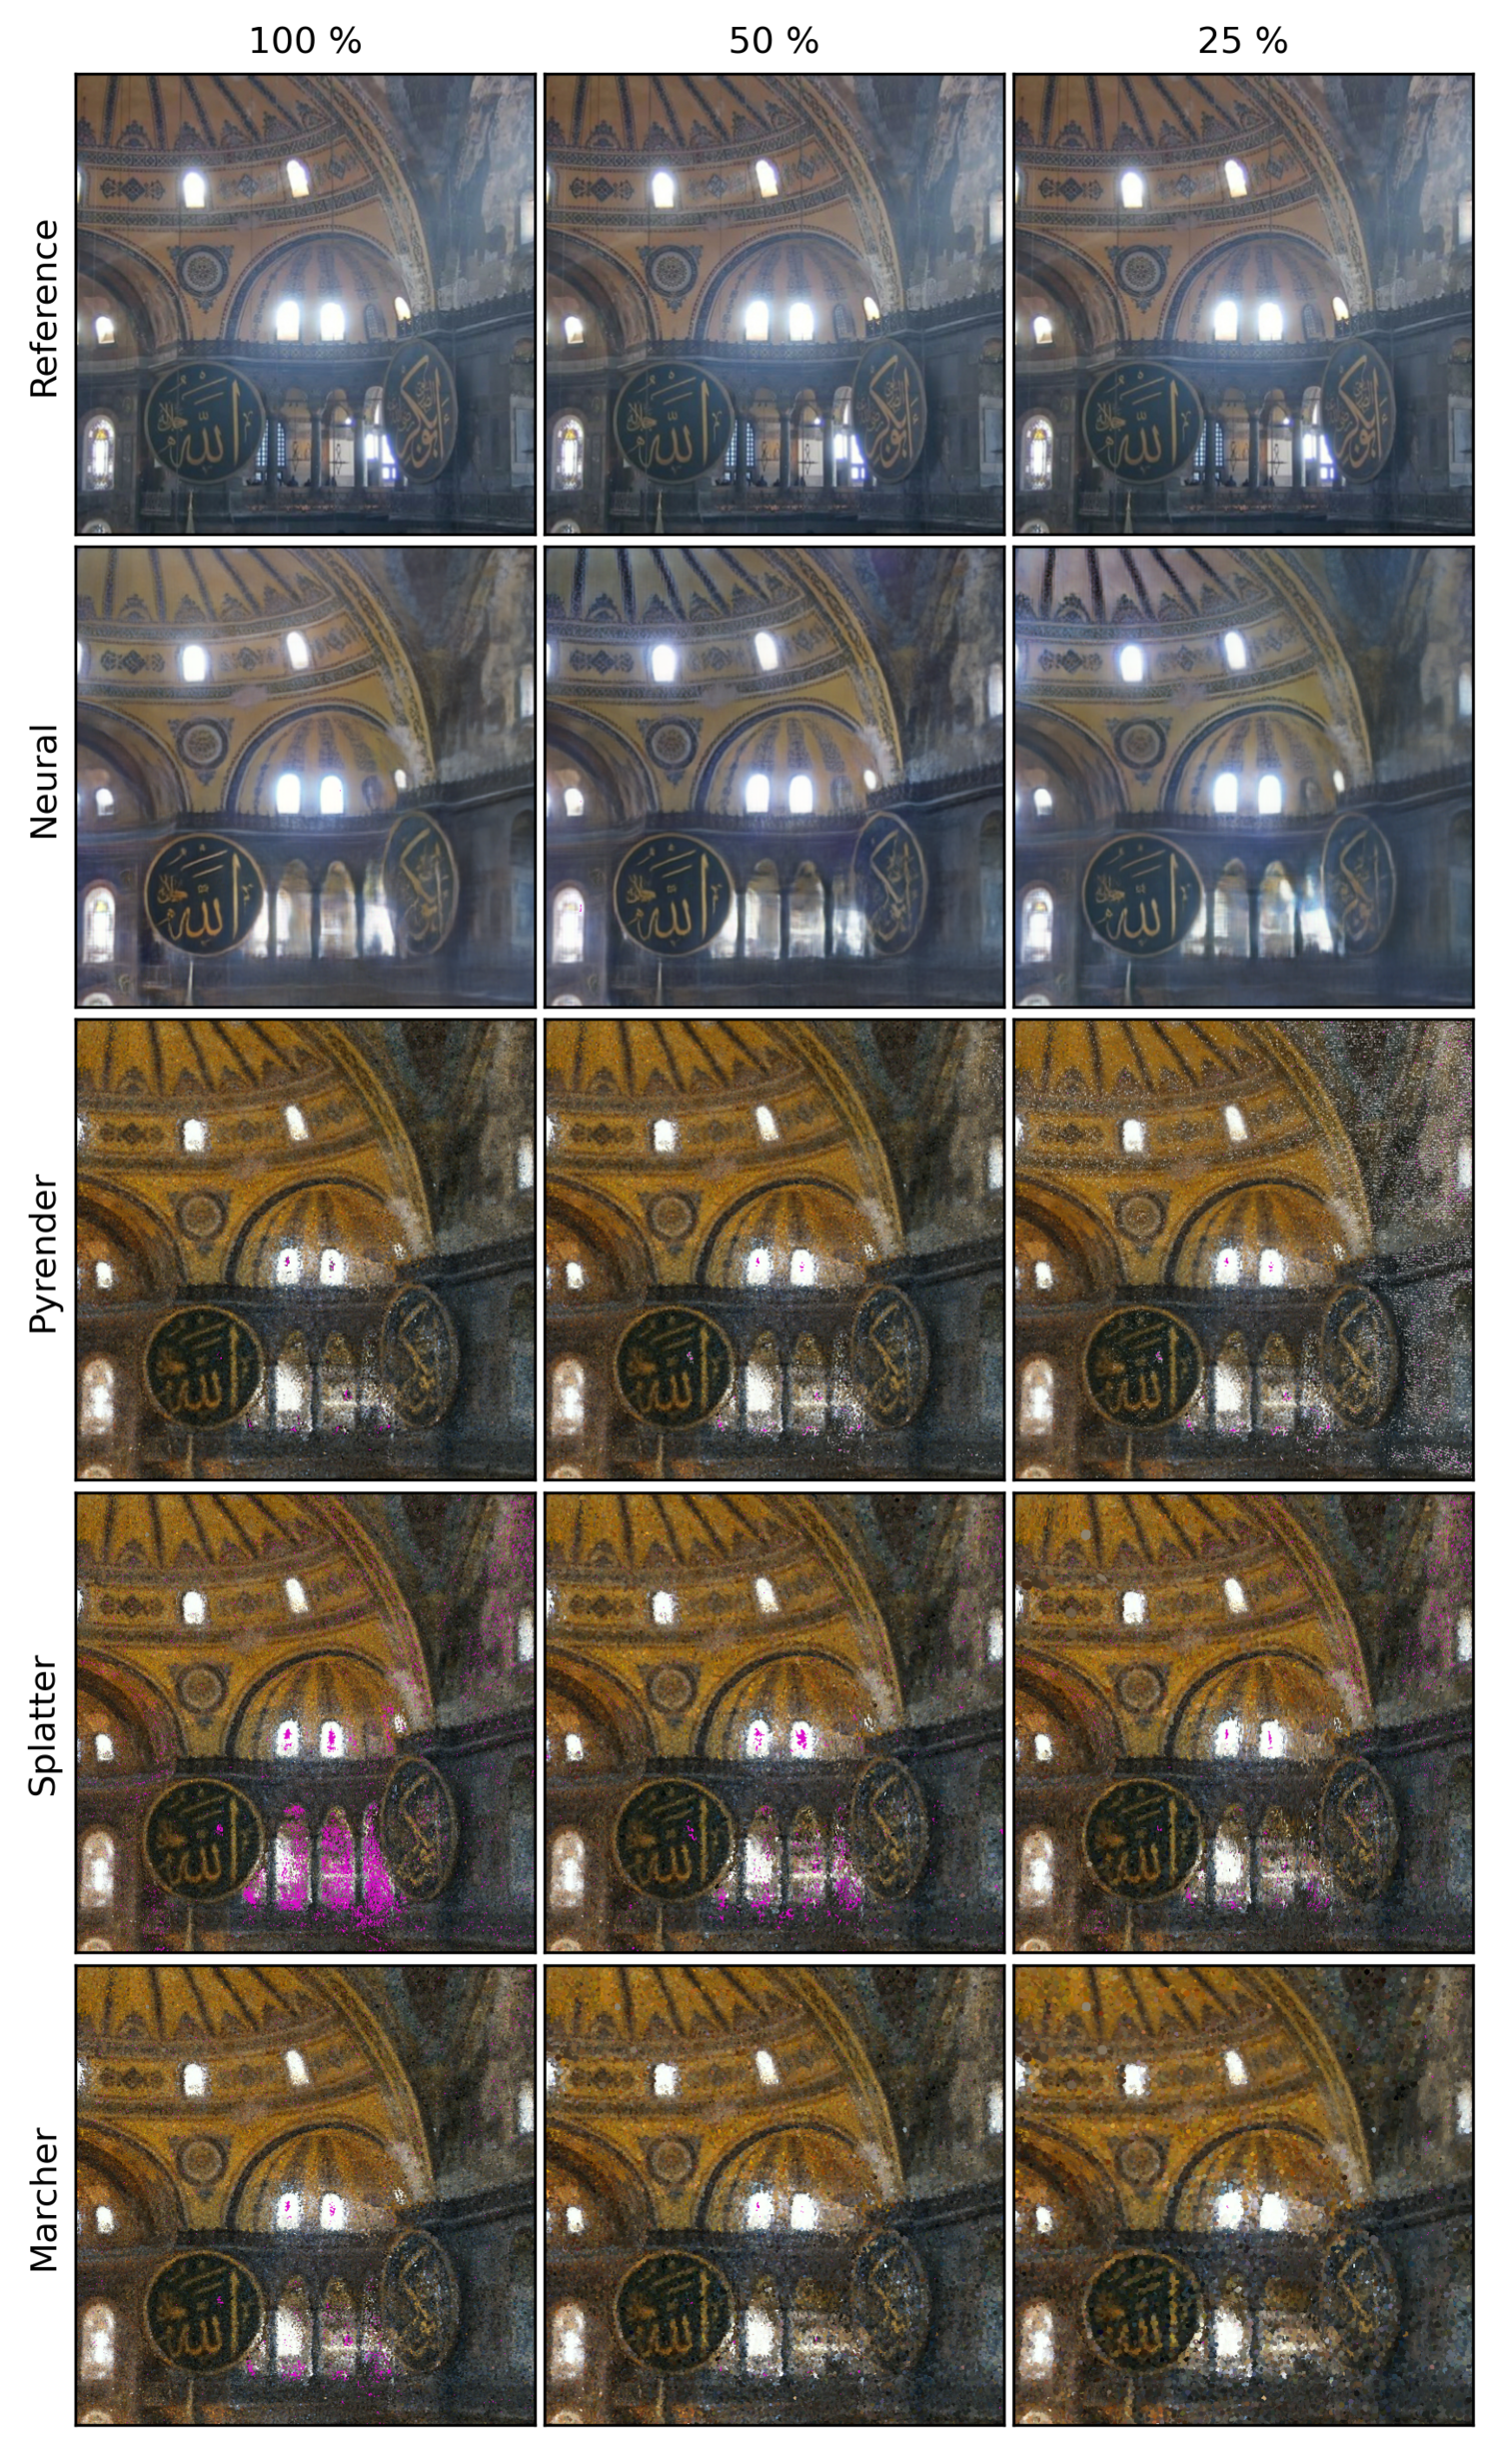
\includegraphics[width=0.9\textwidth]{graphics/hagia-renderers.png}
    \caption[Visual comparison of various renderers and point cloud
    densities for Hagia Sophia Collection]{Visual comparison of various
    renderers and point cloud densities for the Hagia Sophia Collection.
    Contrastive background color is displayed, Open3D's voxel downsampling is used
    for point cloud simplification.}
    \label{fig:hagia_renderers}
\end{figure}

\begin{figure}
    \centering
    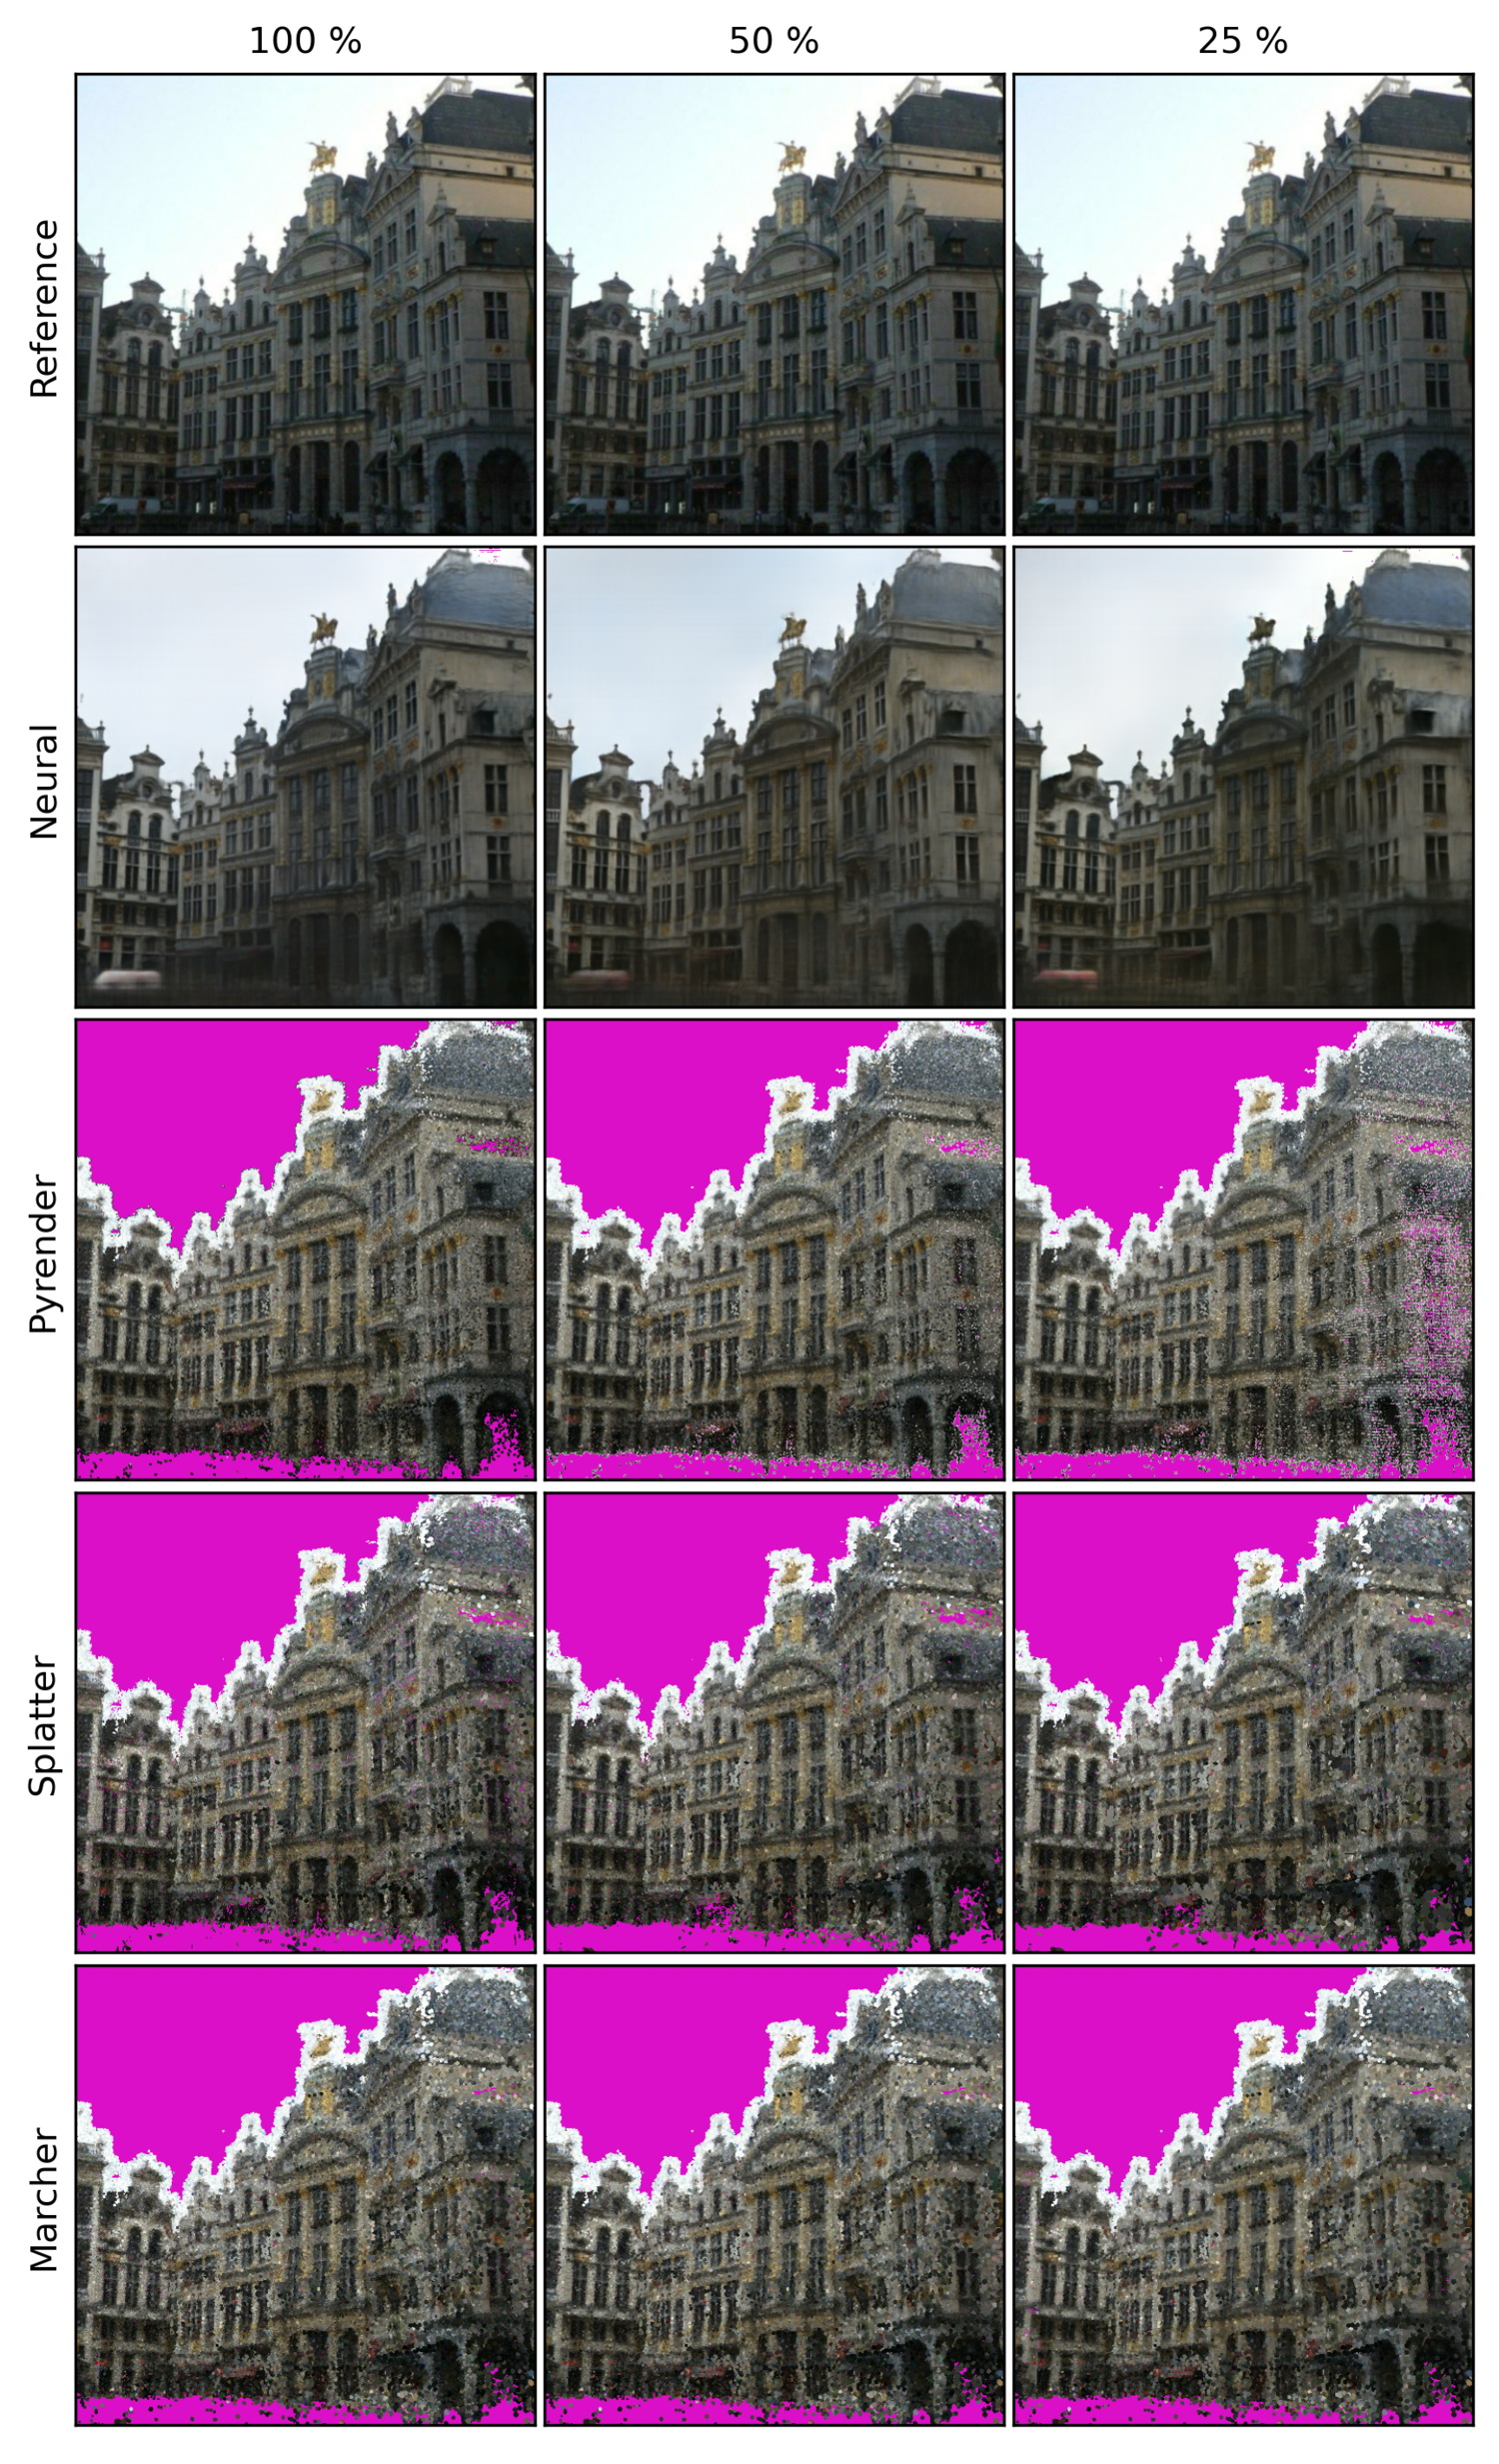
\includegraphics[width=0.9\textwidth]{graphics/grand-renderers.png}
    \caption[Visual comparison of various renderers and point cloud
    densities for Grand Place Brussels Collection]{Visual comparison
    of various renderers and point cloud densities for Grand Place Brussels
    Collection. Contrastive background color is displayed, Open3D's
    voxel downsampling is used for point cloud simplification.}
    \label{fig:grand_renderers}
\end{figure}

\begin{figure}
    \centering
    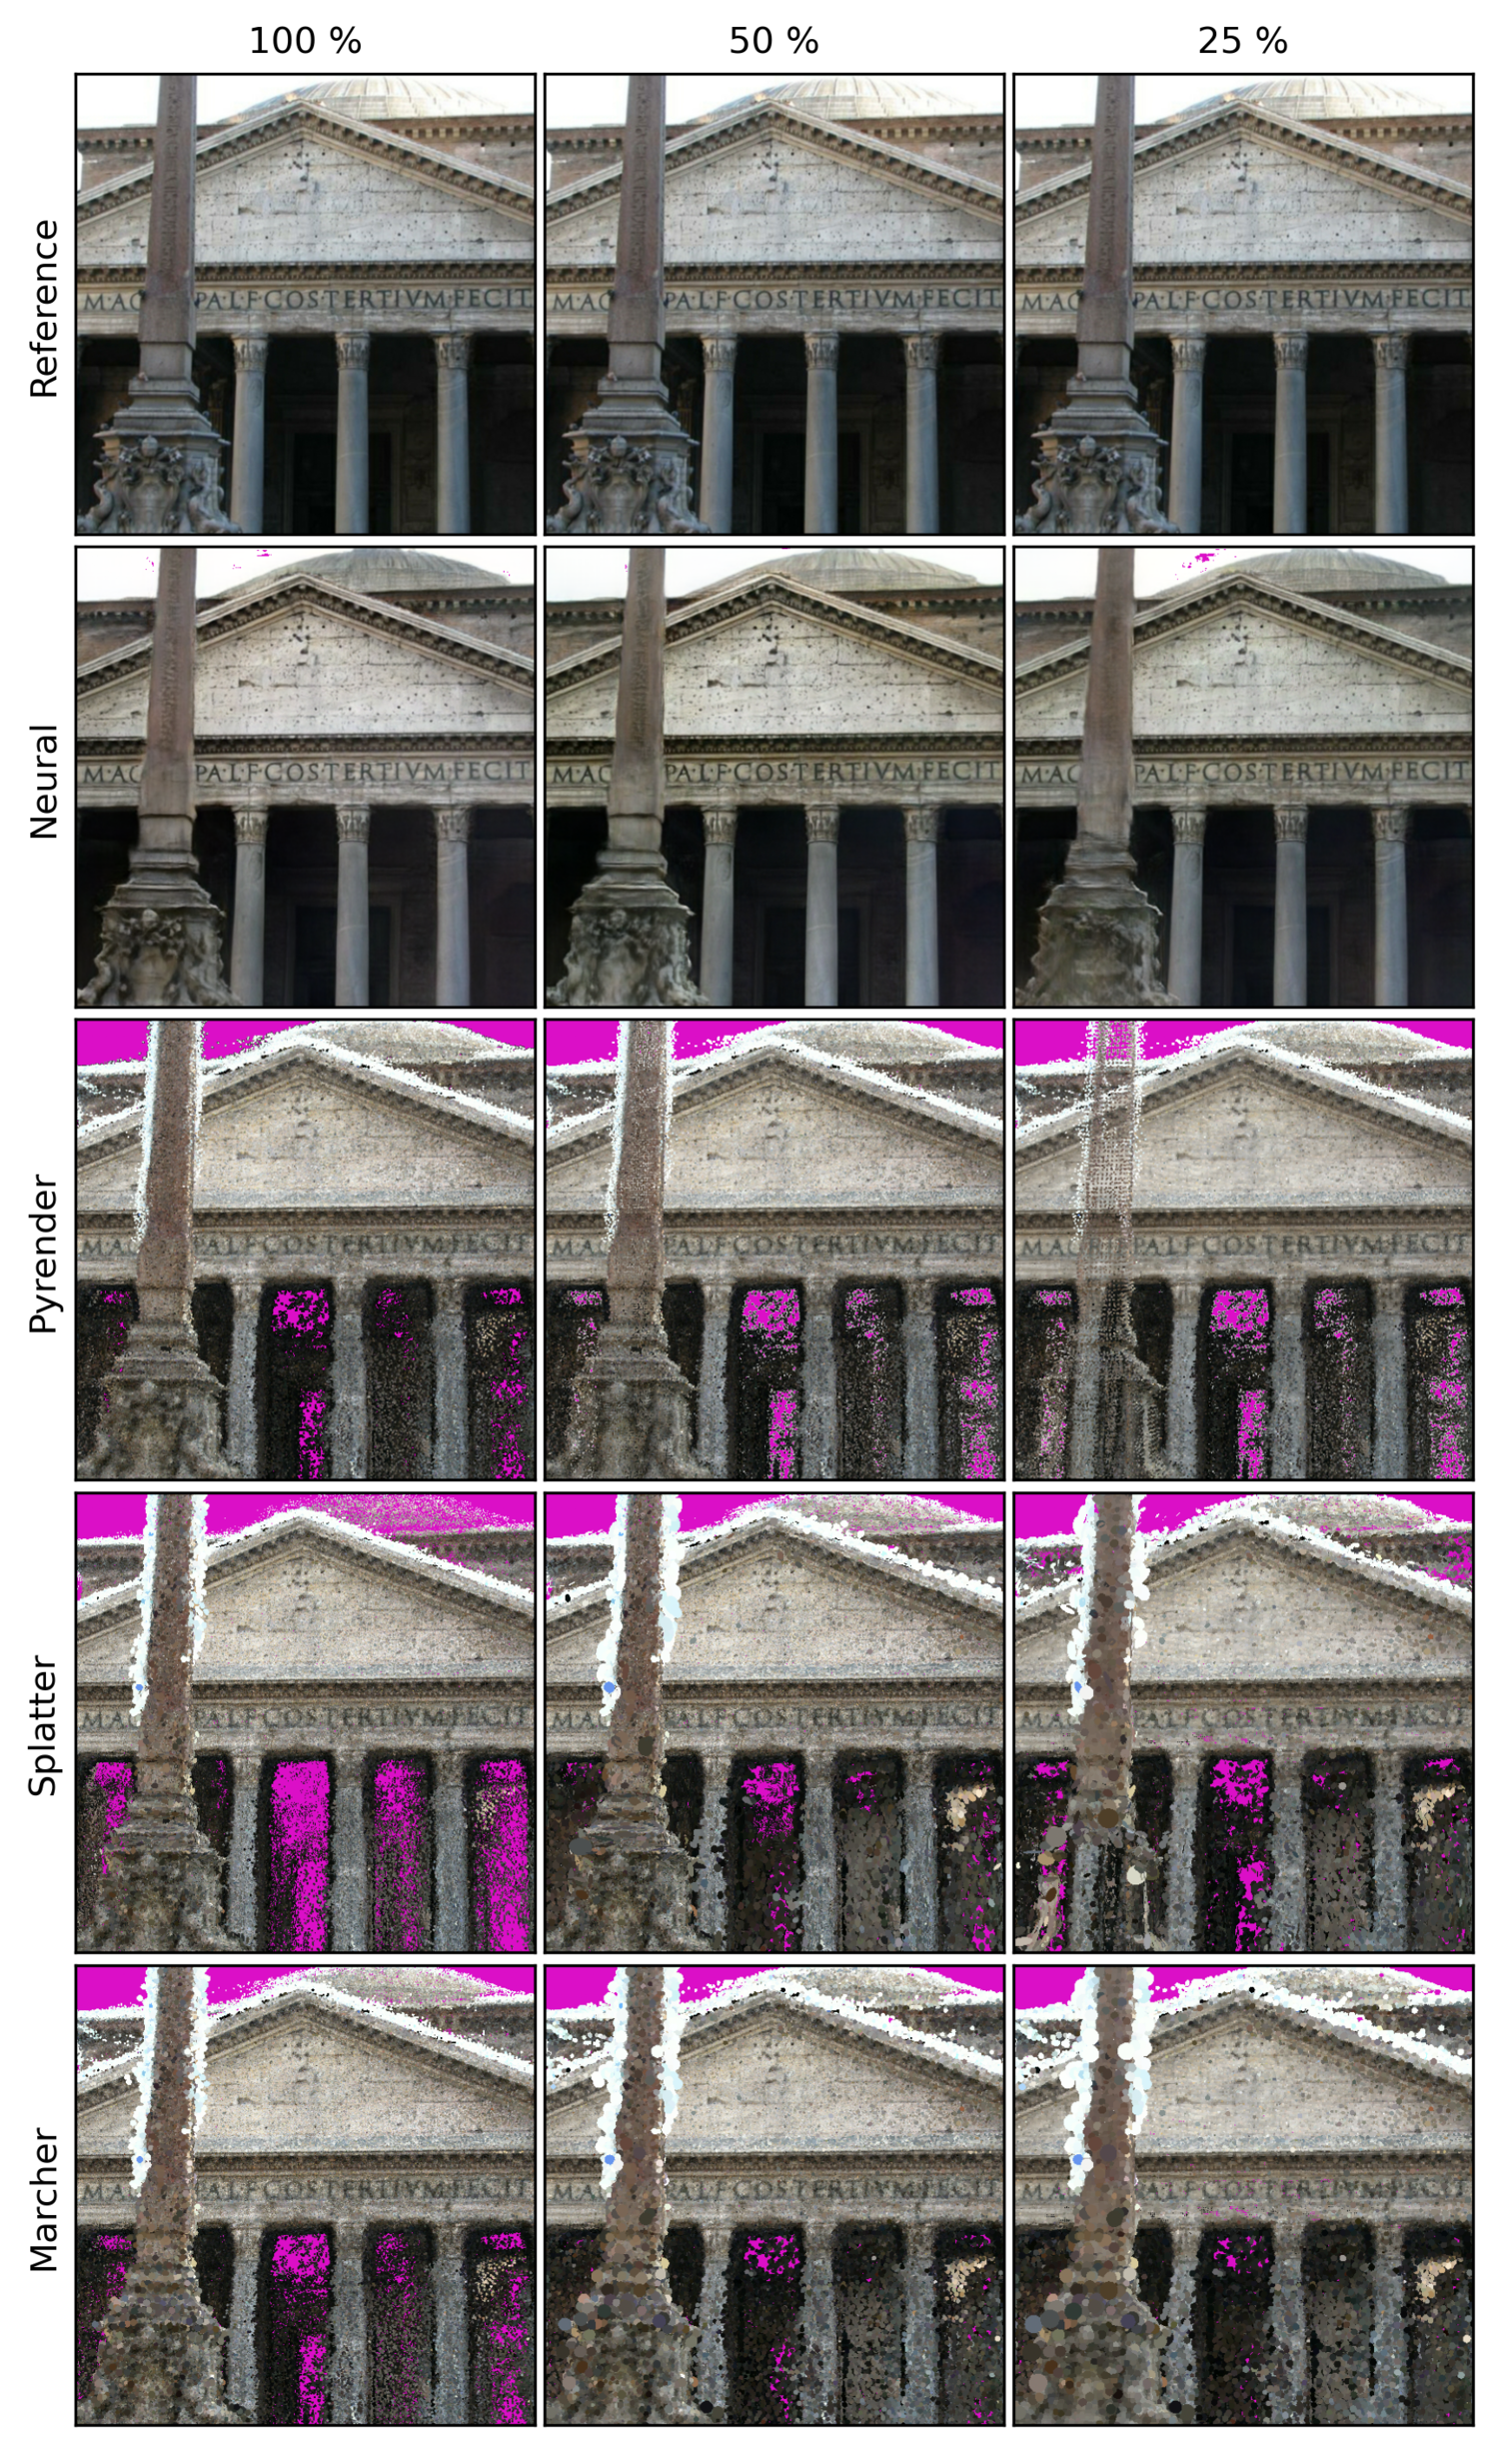
\includegraphics[width=0.9\textwidth]{graphics/pantheon-renderers.png}
    \caption[Visual comparison of various renderers and point cloud
    densities for Pantheon Collection]{Visual comparison of various
    renderers and point cloud densities for Pantheon Collection.
    Contrastive background color is displayed, Open3D's voxel downsampling is used
    for point cloud simplification.}
    \label{fig:pantheon_renderers}
\end{figure}

Influence of training data on NRIW model output is explored
in~\cref{fig:inloc_renderers})\footnotei{.}{As the ARTwin dataset is
not publicly available, it is excluded from visualizations here as its
display is minimized in the thesis.} Two views from the database are displayed
with all non-neural and neural renderers. In the first one with chairs,
one point with a comparatively larger diameter than most others is 
near the left-down corner of the Splatter and Marcher image. These bigger splats
and spheres result in artifacts in neurally-generated images, as 
depicted in the second image row. These patches are something that the screen space
renderer does not suffer from, as all points are of the same screen size.
The advantage of variable diameters
is visible in the second view. With the same sufficient number of points,
the text on the board is more sharp. Also, the floor gets some coverage 
compared to the Pyrender-generated image. The background-filled portions of
Splatter-generated images are caused by the concrete actual point-splatting
implementation, both Splatter and Marcher use the same underlying diameters.\\

\begin{figure}
    \centering
    \includegraphics[width=0.9\textwidth]{graphics/inloc-renderers.png}
    \caption[Visual comparison of various renderers for InLoc dataset]{Visual
    comparison of various renderers for the InLoc dataset.
    For the indoor color profile, the default black background color is contrastive
    enough. The full point cloud was used for the visualizations. In the left-most
    column, repeated reference images for two different views are displayed. In the
    remaining columns, for a given view, up there always is an image generated by
    a non-neural type of renderer below which there is a render generated by NRIW
    trained on the data prepared by the respective non-neural renderer above.}
    \label{fig:inloc_renderers}
\end{figure}

The \textbf{computation rendering performance} relative comparison is
explored in~\cref{tab:render_times}. Relative because computational time
measurements are complex, and in a compute cluster environment that multiple
users actively use, they are also inherently affected by many
external entities. The influence can be alleviated to some extent by using proper
OS time measuring clock type, but it is always better to ideally use the
machine alone for the measuring task, which is hard to ensure on the cluster.
This complexity is to be seen in the table with times varying across
comparable output render dimensions and renderer types.

Across the datasets, the most consistent results are for C++ \emph{Splatter}
implementation. The smallest standard deviations show
implementation consistency. The point cloud size influence is also visible,
as for bigger renders and tens of millions of points, the rendering times
get considerably higher.

The second most consistent results are for
\emph{Pyrender} rendering that internally also uses the standard OpenGL
rendering pipeline and the standard and basic \verb|GL_POINTS| rendering
primitive. Since the implementation wrapper is in Python, we can see much
higher standard deviations.

From the \emph{neural} models, only one is picked for the measurements.
The model size and inference implementation are the same for a dataset, not
depending on the actual rendered data with which the model was trained. The times
are comparable, though the second biggest standard deviations can be seen.
The reason for shorter rendering times for the ARTwin dataset is unclear---the
implementation is in Python, using many software layers underneath, including
NVIDIA driver, so there may be the source of the difference,
alongside demonstrating the complexity of time measurements. The times
are considerably higher compared to those mentioned in the original paper,
but that is to be linked to much higher render dimensions. Moreover, the entire
neural rendering process includes rendering a given point cloud by some
non-neural renderer before inference occurs, which may even double the
rendering time in actual use cases.

C++ implementation of the Marcher does not use the standard OpenGL rendering
pipeline but CUDA parallelization over pixels. Most notably, it
iterates over points in the view frustum, so its rendering computational
performance depends on the 3D structure of a given view of the scene. The
view dependency is  visible in the table, as the standard deviations are
the biggest among renderer types. The implementation may hit some memory
caching or another problem around the InLoc database scan size, as the mean
rendering time and the standard deviation for the InLoc dataset are orders
of magnitude higher than everything else.



\begin{table}
\caption[Mean rendering times]{Measured mean rendering times for the renderers,
collected with the thread CPU time clock, translating to the sum of
the system and user CPU time of the main thread from which rendering is
initiated. It does not include time elapsed during sleep, so it tries to avoid
measuring disturbance from other processes running on the CPU. The clock is
thus a rough approximation of what could be achieved when maximal
performance is sought, and a real-time OS is used. The neural model is not
distinguished here as the model size is the same even though tough weights vary
based on the training data used. The neural rendering time represents solely
the network inference, though preceding it, there must be an aligned triplet
generated, which includes invocation of some non-neural renderer that takes
also some time, as can be seen in the table. The dimension is the biggest
one present in the data being rendered. The measurements were taken on an
Intel Xeon E5-2698 and NVIDIA Tesla V100 GPU.}
\centering
    \begin{tabular}{l c c p{18mm} r r}
    \toprule
    Dataset & Points [M] & Dimension & Renderer & Time [ms] & $\sigma$ [ms] \\
    \midrule
    Hagia Sophia & 5  & 1248 & Neural   & 1\,361 & 139\\
                 &    &      & Pyrender &    783 & 111\\
                 &    &      & Splatter &    156 & 13  \\
                 &    &      & Marcher  & 1\,031 & 397\\[0.3cm]
    Grand Place  & 4  & 1168 & Neural   & 1\,280 & 147\\
                 &    &      & Pyrender &    679 & 82\\
                 &    &      & Splatter &    123 & 7\\
                 &    &      & Marcher  & 1\,448 & 570\\[0.3cm]
    Pantheon     & 5  & 1248 & Neural   & 1\,439 & 156\\
                 &    &      & Pyrender &    857 & 108\\
                 &    &      & Splatter &    173 & 4\\
                 &    &      & Marcher  &    446 & 127\\[0.3cm]
    ARTwin       & 27 & 1600 & Neural   &    871 & 140\\
                 &    &      & Pyrender & 1\,380 & 145\\
                 &    &      & Splatter & 1\,072 & 21\\
                 &    &      & Marcher  &    679 & 382\\[0.3cm]
    InLoc        & 40 & 1600 & Neural   & 1\,749 & 328\\
                 &    &      & Pyrender & 1\,447 & 93\\
                 &    &      & Splatter & 1\,340 & 51\\
                 &    &      & Marcher  & $2\,054\times10^3$ & $1\,684\times10^3$\\
    \bottomrule
    \end{tabular}
\label{tab:render_times}
\end{table}



\subsection{Comparison of localization approaches}

In the localization pipeline, XYZcuts are a vital part of the database
representation based on which a query image pose is calculated. Although
there are XYZcuts present in the InLoc raw dataset, for other datasets explored
in the thesis, they are not. Even for the InLoc dataset, some misalignments
are hidden in verified scan poses, also noted in the InLoc
algorithm Github repository issue. Thus, a way of computing this 3D data
representation is devised and applied to all datasets, including the InLoc one.
The process poses dependence of the localization
pipeline on a non-neural renderer---as specified in~\nameref{subsec:inloc},
the XYZcut is computed utilizing the depth map produced by a renderer per
localization database image. The depth map is used to transform
per-pixel 3D points placed on a default plane in the distance of one from a camera
center perpendicular to the given database image camera's optical axis.\\

In this section, three concepts are thus examined. Firstly, the influence
of a non-neural renderer-based database representation on the whole
localization process is explored on IMC image collections, end-to-end. Secondly,
the influence of given database representation with fixed pose verification step
renderer, including neural ones, on the localization performance is inspected
on ARTwin data. Finally, the influence of solely pose verification renderer
choice for one fixed database representation is considered for the InLoc dataset.\\

In~\cref{tab:imc_inloc_performance}, we can explore the localization on IMC
image collection from the smallest datasets on top to the biggest at the bottom of the
table. The overall rates of correctly localized queries are much smaller
compared to ARTwin and InLoc data. That may be caused by the combination of
three factors---several folds smaller dataset sizes; varying database image
dimensions, some of which are as small as 100~pixels in each dimension; varying
sensor types, sizes, and all adversarial effects of manual acquisition, such as
extensive blur. The absolute error sizes, when compared to the size of the
scene models, are relatively still small because, contrary to the other two
datasets, IMC data cover enormous external or internal spaces over much
bigger scale than mostly close looks at either manufacturing equipment or
corridors and other, in nature, office spaces.

The table shows that the splatting InLoc variant is predominantly the
most precise one with the most outliers on smaller precision thresholds
among the smallest Hagia Sophia collection. The second most precise
localization variant seems to be the Pyrender one. However, we will see that
comparison to the marching variant may be affected by a small dataset
size. The medians and means of Euclidean and angular distances support the
thesis of database size influence on localization performance (aside from the
simple idea that more database images mean a higher chance of retrieving one
captured more closely, thus triangulating a more precise pose). The bigger
the dataset size is, the smaller these statistics are. Also to be noted is the
fact that having fewer database images to perform the image retrieval has a
bigger influence on angular precision than Euclidean one.\\



\begin{table}
\caption[InLoc performance on IMC collections]{Evaluation
of localization performance on IMC collections using the InLoc
pipeline fully based on a given type of non-neural renderer,
including the pose verification step. The performance is
constituted by a percentual rate of correctly localized queries
at a given precision threshold. General statistics of calculated poses
in the form of mean and standard deviation for distance and
angular distance are also displayed.}
\centering
    \begin{tabular}{c c S[table-format=3.2] S[table-format=3.2] S[table-format=3.2] }
    \toprule
    Collection & Precision\,$+$\,Statistics & {Pyrender} & {Splatter} & {Marcher} \\
    \midrule
    Hagia Sophia
    & $\D2.50\m,\D7.5\dg$ &  \B{2}    &     0     &     0    \\
    & $\D5.00\m, 10.0\dg$ &  \B{4}    &  \B{4}    &     2    \\
    & $\D7.50\m, 15.0\dg$ &    18     &    16     & \B{20}   \\
    & $ 10.00\m, 20.0\dg$ & \B{52}    &    44     &    50    \\
    & $ 15.00\m, 30.0\dg$ &    86     & \B{90}    & \B{90}   \\
    & $ 20.00\m, 30.0\dg$ &    86     & \B{90}    & \B{90}   \\
    & Median [$\M$]       &     2.44  &  \B{2.10} &     2.37 \\
    & $\sigma$ [$\M$]     &     2.07  &  \B{1.80} &     2.21 \\
    & Median [$\dg$]      & \B{19.88} &    20.28  &    20.07 \\
    & $\sigma$ [$\dg$]    &    21.09  & \B{19.50} &    21.42 \\[0.3cm]
    Grand Place
    & $\D2.50\m,\D7.5\dg$ &     2    & \B{4}     &     2    \\
    & $\D5.00\m, 10.0\dg$ &     8    & \B{8}     &     6    \\
    & $\D7.50\m, 15.0\dg$ &    38    & \B{46}    & \B{46}   \\
    & $ 10.00\m, 20.0\dg$ &    72    & \B{76}    &    74    \\
    & $ 15.00\m, 30.0\dg$ & \B{90}   &    88     &    88    \\
    & $ 20.00\m, 30.0\dg$ & \B{90}   &    88     &    88    \\
    & Median [$\M$]       &     1.63 &  \B{1.50} &     1.75 \\
    & $\sigma$ [$\M$]     &     2.17 &  \B{1.45} &     2.29 \\
    & Median [$\dg$]      &    16.29 & \B{15.65} &    15.84 \\
    & $\sigma$ [$\dg$]    &    23.71 & \B{19.18} &    27.89 \\[0.3cm]
    Pantheon
    & $\D2.50\m,\D7.5\dg$ &     14     & \B{26}   &    22    \\
    & $\D5.00\m, 10.0\dg$ &     34     & \B{44}   & \B{44}   \\
    & $\D7.50\m, 15.0\dg$ &     72     & \B{82}   & \B{82}   \\
    & $ 10.00\m, 20.0\dg$ &     88     & \B{92}   &    90    \\
    & $ 15.00\m, 30.0\dg$ & \B{100}    &    98    &    96    \\
    & $ 20.00\m, 30.0\dg$ & \B{100}    &    98    &    96    \\
    & Median [$\M$]       &      1.50  & \B{1.09} &     1.48 \\
    & $\sigma$ [$\M$]     &      3.24  & \B{1.79} &     3.02 \\
    & Median [$\dg$]      &  \B{10.04} &   11.99  &    10.52 \\
    & $\sigma$ [$\dg$]    &     21.80  & \B{5.44} &    19.08 \\
    \bottomrule
    \end{tabular}
\label{tab:imc_inloc_performance}
\end{table}


Considering fixing the pose verification step and observing localization
performance with varying database representations,
\cref{tab:artwin_inloc_performance} presents the results on the ARTwin
dataset. The general positive impact of using neural rendering
approach for pose verification is shown. Across the pose verification
variants, the radii-based renderers perform better than the Pyrender ones,
no matter whether neural or non-neural variant is considered. This further
support the claim that better training data generation process positively affects
neural model performance, though the percentual margin may not be that
significant as these models can compensate for many imperfections in the
deep buffer.

Further, for the candidate pose generation InLoc localization
pipeline part, with a bigger dataset the marching-based InLoc Base variant
shows its better performance rather closing to the splatting variant, both
outperforming the Pyrender variant. From a median error point of view,
having a bigger dataset is also beneficial. The mean of median Euclidean
distance errors across the table is only $0.26\m$, and the mean of median
angular distance errors is as low as only $0.64\dg$. These results
are much better compared to those obtained on IMC collections, but as
described in the paragraphs devoted to~\cref{tab:imc_inloc_performance},
ARTwin dataset consists of more database images with the same dimensions,
consistent quality, and sensor parameters ensured by the image acquisition
process. The scanner used for dataset generation uses more \uv{normal} 2D
cameras to create $360\dg$ RGB scans, so when the InLoc database is created,
there are sometimes visible minor artifacts of this two-way process. An example
of such an artifact together with localization visualization is
in~\cref{fig:artwin_loc}. In the light of such minor defects, the absolute
errors are even more impressive.


\def\idone{$0.25\m, 2\dg$}
\def\idtwo{$0.50\m, 5\dg$}
\def\idthree{$5.00\m, 10\dg$}
\begin{table}
\caption[Pose verification performance on ARTwin dataset]{Evaluation
of localization performance on the ARTwin dataset. The performance is
constituted by a percentual rate of correctly localized queries
at a given precision threshold. InLoc Base refers to a renderer type on
which the localization database is constructed, pose verification renderer
is denoted as \emph{P} (Pyrender), \emph{S} (Splatter), \emph{M} (Marcher),
and three \emph{N} variants standing for NRIW trained on training data
generated by the respective renderer.}
\centering
    \begin{tabular}{l c S[table-format=3.2] S[table-format=3.2] S[table-format=3.2] }
    \toprule
    Pose Verification & InLoc Base & {\idone} & {\idtwo} & {\idthree} \\
    \midrule
    P   & Pyrender &    40.0  &    48.7  &    62.7  \\
        & Splatter & \B{40.1} & \B{49.9} &    62.6  \\
        & Marcher  &    39.9  &    49.2  & \B{63.1} \\[0.3cm]

    S   & Pyrender & \B{41.2} &    51.4  &    62.8  \\
        & Splatter &    40.0  &    53.3  & \B{64.7} \\
        & Marcher  &    40.9  & \B{53.5} &    63.9  \\[0.3cm]

    M   & Pyrender &    41.0  &    50.7  &    65.3  \\
        & Splatter & \B{42.1} & \B{53.1} & \B{65.8} \\
        & Marcher  &    41.3  &    52.7  &    65.5  \\[0.3cm]

    N-P & Pyrender &    43.8  &    51.9  &    68.3  \\
        & Splatter &    44.0  &    51.8  & \B{70.1} \\
        & Marcher  & \B{44.2} & \B{52.8} &    69.2  \\[0.3cm]

    N-S & Pyrender &    45.6  &    55.1  &    72.7  \\
        & Splatter & \B{45.9} &    59.3  &    73.4  \\
        & Marcher  &    45.7  & \B{59.5} & \B{74.6} \\[0.3cm]

    N-M & Pyrender &    45.9  &    55.0  &    71.9  \\
        & Splatter &    46.2  & \B{60.5} &    73.8  \\
        & Marcher  & \B{47.2} &    58.9  & \B{74.7} \\
    \bottomrule
    \end{tabular}
\label{tab:artwin_inloc_performance}
\end{table}

\begin{figure}
    \centering
    \begin{subfigure}{.95\textwidth}
          \centering
       \includegraphics[width=.95\textwidth]{../graphics/err_0.01m_0deg_results_q_id_3_best_db_1}
    \end{subfigure}%
    
    \begin{subfigure}[width=.95\textwidth]{.95\textwidth}
          \centering
          \includegraphics[width=.95\textwidth]{../graphics/err_0.18m_1deg_results_q_id_137_best_db_1}
    \end{subfigure}
    \caption[Sample localization visualizations]{The first column shows the
    query photo, the second render of the best candidate position, the third
    a blend of the two preceding columns and the last column shows the
    database photo obtained from the image retrieval step. The upper row
    shows an error of $0.01\m$ and $0\dg$, the second an error of $0.18\m$
    and~$1\dg$. On the query image of the second row, there is also visible
    the relic of the reprojection from panorama photo to 2D photo on the tubes
    in the foreground.
    }\label{fig:artwin_loc}
\end{figure}



% \begin{figure}
%     \centering
%     \includegraphics[width=.95\textwidth]{graphics/correctly_localized_queries}
%     \caption[]{}
%     \label{fig:artwin_loc_graph}
% \end{figure}


Finally, for the InLoc dataset, the results are presented
in~\cref{tab:inloc_performance}. The percentual rates are comparatively
worse than the one from previous research; the reason is that I faced
a lot of issues around the InLoc dataset, including the mentioned skewed
database positions, and I was not able to resolve it properly.
Though lower in absolute numbers, the distortion is the same across
all results; thus, the relative comparisons still pose valuable insights.
Based on the outcomes of preceding experiments, with fixed localization
dataset generation via splatting, we compare the performance of various
pose verification approaches with \url{https://www.visuallocalization.net}.

For the InLoc dataset, the Marcher renderer performs best, outperforming
both remaining non-neural renderers. The dominance over this dataset
gets translated over to neural models as well. Even more than in the case
of the ARTwin dataset, we can see the benefit of neural rendering in this
case: ray marching varies between 7.1~\% to 9.1~\% for three precision
thresholds. All three neural models show a positive impact over non-neural
variants.

The splatting-based variants are the least performing among others on this
dataset. The reason may be hidden in Lipponer's implementation, as
some artifacts are visible in~\cref{fig:inloc_renderers}. That may
arise from the number of points in the scan, as it is the highest among all
the datasets in the thesis, or the format of the scans themselves, generated
by Matlab in the raw dataset data and later transformed into PLY file format.

Although there was this headache with the InLoc dataset, radii-based renderers
shown their value and benefits over all datasets, as well as neural rendering
that further pushes localization performance rates.



\begin{table}
\caption[InLoc performance on InLoc dataset]{Percentual rate of
correctly localized query images within the displayed distance
and angular distance for the DUC1 floor. The table explores the behavior
of fixed candidate positions localization part and multiple
pose verification rendering methods denoted as \emph{P} (Pyrender),
\emph{S} (Splatter), \emph{M} (Marcher), and three \emph{N} variants
standing for NRIW trained on training data generated by the respective
renderer.}
\centering
    \begin{tabular}{c S[table-format=3.2] S[table-format=3.2] S[table-format=3.2] | S[table-format=3.2] S[table-format=3.2] S[table-format=3.2] }
    \toprule
    Rate [\%]           & {P}  & {S}  & {M}     & {N-P} & {N-S} & {N-M} \\
    \midrule
    $\D0.25\m,\D2.0\dg$ & 22.2 & 19.2 & \B{22.7} & 26.8 & 21.2 & \B{29.8} \\
    $\D0.50\m,\D5.0\dg$ & 28.3 & 26.3 & \B{30.3} & 31.8 & 24.2 & \B{38.9} \\
    $\D5.00\m, 10.0\dg$ & 37.4 & 36.4 & \B{41.9} & 43.4 & 31.8 & \B{51.0} \\
    \bottomrule
    \end{tabular}
\label{tab:inloc_performance}
\end{table}
